\section{Structural model}
\label{sec:structuralModel}
This section deals with the first term of the right hand side in eq.\ref{eq:nlmeModel}
\begin{align*}
	f(x_{ij}, \psi_{i}) 
\end{align*}
i.e. the model prediction.

It can be formulated as a simple algebraic equation (e.g. Hill equation) or complex physiology-based PK model implemented as system of ODEs. When defined in such framework, this deterministic model for an individual will later be embedded in a statistical model. Other approaches, such as SDE-based structural models are not supported in this specification.

%\begin{figure}[htbp]
%\begin{center}
%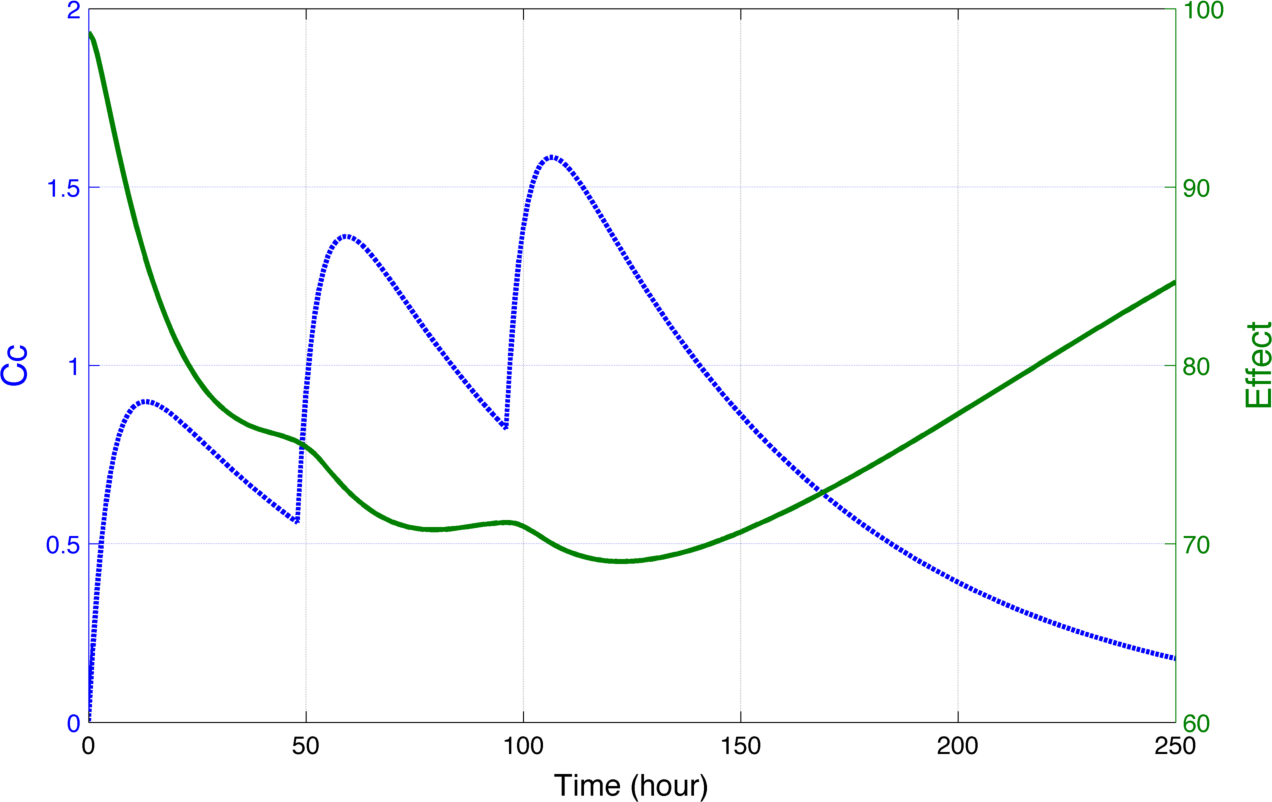
\includegraphics[width=.45\textwidth]{CTS1_smallPKPD}
%\caption{Simulated combined model as defined in the example with PK (blue) and PD (green) time courses for one subject. Here three doses were administered every $48h$.}
%\label{fig:simplePKPD}
%\vspace{-20pt}
%\end{center}
%\end{figure}
%  \vspace{-20pt}
%  \caption{A gull}
%  \vspace{-10pt}
%\end{wrapfigure}
\paragraph{Example}
As an example of a structural model we consider a combined PK/PD model, % see figure \ref{fig:simplePKPD},
\begin{itemize}
\item
PK -- oral one-compartmental model
\item
PD -- turnover model, so called $I_{max}$ model
\end{itemize}
with the following model parameters $ka$, $V$, $CL$, $Imax$, $IC50$, $Rin$ and $kout$.
\begin{align*}
k&=CL/V  \\
\frac{dAd}{dt} &=-ka\times Ad  \\
\frac{dAc}{dt}&=ka \times Ad - k \times Ac  \\
\frac{dE}{dt}&=Rin \times \Bigg(1-\frac{Imax \times Cc}{Cc+IC50}\Bigg) - kout \times E \\
\mbox{Initial condition: } & E(t=0) = Rin/kout   \\
& Ad(t=0) = DoseSize  \\
& Ac(t=0) = 0;  \\
Cc &= Ac/V  
\end{align*}

\paragraph{Alternative formulation}
The PK model can, in this case, be formulated as an algebraic equation because an analytic solution exists, i.e.
\begin{align*}
C(t) = \frac{D}{V}  \frac{ka}{ka - k} \Big(e^{-k(t-t_D)} - e^{-ka(t-t_D)} \Big) 
\end{align*}

\subsection{Delayed Differential Equations (DDE)} % {\color{red} \scshape{***** NEW *****}}
Additionally to the ODEs and algebraic equations, version \currpml of PharmML offers
the possibility to use Delayed Differential Equations. Similarly to initial conditions required
for an ODE, the so-called \emph{history} has to be defined. If a model is defined for times
$t \geq t_0$, the history specifies the values of the model variables for the 
time $\leq t_0$. 
The following simple example, from \cite{MLXTRANforMonolix:2014}, shows how 
such model and the according history can be formulated. 
\begin{align}
& \frac{dA}{dt} = r - c \times A \times B - k \times A \nonumber \\
& \frac{dB}{dt} = c \times A \times B - A(t-d) \nonumber 
\end{align}
with history $A_0 = r/k$ and $B_0 = 0$ for $t \le 5$. \emph{d} is the discrete delay parameter.

%
%\begin{eqnarray}
%\frac{d\textbf{y}(t)}{dt} &=& F(t,\textbf{y}(t)) \nonumber \\
%with  && \textbf{y}(t_0) = \textbf{y}_0  \nonumber
%\end{eqnarray}
%
%i.e. using explicit, first order ODEs.
%
%\paragraph*{Note on initial conditions}
%Some models have long algebraic expressions for every initial condition, e.g. here the value for glucose in liver:
%\begin{eqnarray}
%G_{L,0}=(1/Q_{G,L})*(Q_{G,A}*G_{H,0} + Q_{G,G}*G_{G,0} + Q_{G,PN}*G_{PN,0} + r_{B_{HGP}} - r_{B_{HGU}}) \nonumber
%\end{eqnarray}
%with 
%Initial conditions (defined/calculated before)
%\begin{eqnarray}
%&&G_{H,0} = a; \;\;\;G_{G,0} = b; \;\;\;G_{PN,0} = c; \quad with \quad a,b,c \in R \nonumber 
%\end{eqnarray}
%and other user defined functions
%\begin{eqnarray}
%&& r_{B_{HGP}} = f_1(y) \nonumber \\
%&& r_{B_{HGU}} = f_2(y) \nonumber
%\end{eqnarray}

